\pagenumbering{arabic}
\section{Introduksjon}

Helse Nord IKT er et eget foretak under Helse Nord paraplyen som i hovedsak leverer tjenester til andre foretak i Helse Nord. Seksjon for systemutvikling i avdeling for Tjenesteutvikling er delt opp i ulike team. 

\subsubsection*{Kvalitetsregister}

Denne oppgaven er på bestilling fra team for kvalitetsregister. Helse Nord IKT er en av to godkjente leverandører av nasjonale medisinske kvalitetsregister. Teamet jobber med å utvikle plattform for kvalitetsregister samt de spesifikke register.

Kvalitetsregister som utvikles av HN-IKT:
\begin{itemize}
    \item Norsk gynekologisk endoskopiregister\cite{1-kvalitetsregistre.no}
    \item Norsk register for invasiv kardiologi\cite{1-ablanor}
    \item Norsk kvalitetsregister for behandling av spiseforstyrrelser\cite{1-Norspis}
    \item Norsk register for arvelige og medfødte nevromuskulære sykdommer\cite{1-muskel}
    \item Norsk register for analinkontinens\cite{1-nra}
    \item Norsk register for gastrokirurgi\cite{1-norgast}
    \item Norsk kvalitetsregister for endokarditt\cite{1-endokarditt}
    \item Nasjonalt register for ablasjonsbehandling og elektrofysiologi i Norge (AblaNor)\cite{1-ablanor}
    \item Nasjonalt register for langtids mekanisk ventilasjon LTMV\cite{1-langmek}
    \item Norsk kvalitetsregister for fedmekirurgi (SOReg-Norge)\cite{1-soreg}
    \item Nasjonalt kvalitetsregister for ryggkirurgi (Paraply for tre register - Deformitet/Rygg/Nakke)\cite{1-rygg}
\end{itemize}

Et medisinsk kvalitetsregister er en registrerings løsning for medisinske data relatert til et spesifikt fagfelt, der data samles inn for å brukes til forskning. Et eksempel på et slikt register er Norsk Gynekologisk Endoskopi Register(NGER).

Registeret samler inn data om \cite{1-kvalitetsregistre.no}:

\begin{itemize}    
    \item Konvertering til laparoskopi (ut fra hysteroskopi)/ laparotomi (ut fra hysteroskopi, laparoskopi)
    \item Intraoperative komplikasjoner
    \item Postoperative komplikasjoner
    \item Reoperasjon for komplikasjoner innen 4 uker
    \item pasientens helsegevinst og 
    \item tilfredshet med behandlende enhet
\end{itemize}

Ved å samle inn data fra alle pasienter som blir endoskopisk operert for gynekologiske tilstander og sykdommer ved offentlige og private sykehus er det da mulig å utføre statistiske analyser for å identifisere positive og negative aspekter ved det enkelte behandlingssted og på tvers av behandlingssted \cite{1-kvalitetsregistre.no}.  

På denne måten er nasjonale kvalitetsregister et viktig verktøy for å sikre lik og trygg behandling for alle pasienter uavhengig av geografisk tilhørighet.

Data samlet inn via slike medisinske kvalitetsregistre danner grunnlag for analyse og forskning som har som formål å gi økt behandlings kvalitet
ved norske sykehus. Innregistrering av data til medisinske kvalitetsregistre blir ofte utført av helsepersonell, ofte i en hektisk hverdag der de har
mange andre arbeidsoppgaver. Det er av den grunn viktig at det er mulig å utføre registrering av data på en enkel måte med liten risiko for feil.
Forbedring av kvalitet skjer ofte via kvalitets-forbedringsprosjekter. \cite{1-kvalitetsforbedring}.  

Helse Nord IKT leverer en plattform for medisinske kvalitetsregister som er basert på OpenQReg. OpenQReg er utviklet i Sverige av Uppsala Clinical Research Center.\cite{Jernberg1617} OqenQReg er en av tre godkjente plattformer for medisinske kvalitetsregister i Norge.
Teamet jobber med å utvikle plattform for kvalitetsregister samt de spesifikke register som bruker plattformen.\cite{1-norsk-helsenett}  

OpenQreg plattformen er opprinnelig utviklet av Uppsala Clinical Research Centre som en åpen basis plattform for kvalitetsregistre. HN-IKT har nå sin egen "fork" av denne som vedlikeholdes og videreutvikles.

\subsection{Bakgrunn for oppgaven} 

For registrering av medisinske kvalitetsparametre brukes det diverse kodeverk.
Et praktisk eksempel på et kodeverk vi alle kjenner er postnummer. Et postnummer er en lenke til informasjon om et sted, den inneholder informasjon om hvilket fylke og by det referer til.
Postnummer er et av kode-verkene applikasjonen skal omfavne. Den skal også omfavne medisinske kodeverk. De kobler en kode opp mot en diagnose eller tilstand.

Kodeverk som brukes er:
\begin{itemize}
   \item Postnummer
   \item ICD10 \cite{1-ICD-10}
   \item NCMP \cite{1-NCMP}
   \item NCSP \cite{1-NCSP}
\end{itemize}

Dette er i dag opplysninger som er hard kodet inn i applikasjonens database, og som lastes inn ved oppstart av applikasjonen.
Det er også andre kodeverk som er ønsket av registrene, men som ennå ikke er inkludert i applikasjonen.

Med dagens løsning kan hvert enkelt kvalitetsregister oppdage at diverse koder eller dokumenter ikke er oppdatert til nyeste versjon. Dette fører til
at data ikke kan registreres korrekt av helsepersonellet som utfører registreringen. Når en sluttbruker oppdager dette vil den ta kontakt med
utviklerne via felles epost portal, en utvikler vil så opprette SQL script for oppdatering til nye koder. Dette scriptet sendes til driftspersonell
som så kjører scriptet i produksjonsdatabasen. Prosessen gjentas for alle 13 kvalitetsregistre. Dette er en ugunstig prosess da den stjeler tid
fra sluttbruker og utviklere.

Det er derfor ønskelig med en felles tjeneste som kan hente inn koder fra ulike kilder (API, filer osv.) sammenfatte og versjons styre kodene. For
så å levere de til register applikasjonene via et REST API. Det er altså ønskelig automatisere oppdatering prosessen i størst mulig grad,
og på denne måten kunne tilby mest mulig oppdatert data. Dette vil være til gevinst for både sluttbruker og for utviklere.

Det er da også naturlig at det implementeres en klient til APIet i registrenes felles kode. Da er det naturlig å tenke at
koder ikke lengre lagres i SQL databasen, men heller i en type in-memory database for raskere oppslag i applikasjonen.
In-memory databasen settes opp slik at den oppdateres hver gang det kommer nye koder i REST APIet.

Det er også uttrykt et ønske om mulighet for laste versjonsstyrte dokumenter inn i applikasjonen som kan lagres som binary
blobs. De skal også tilgjengeliggjøres via APIet. Dette ønskes da hvert kvalitetsregister lagrer og gjør tilgjengelig et antall
dokumenter for ulike formål. Det lagres også maler for meldinger som skal sendes til innbyggere. Det er da ønskelig å ha en
felles portal for å oppdatere disse dokumentene.

En siste årsak til ønske om en felles tjeneste for dokumenter og kodeverk er alderen og den akkumulerte tekniske gjelden i OpenQReg plattformen. For å kunne vedlikeholde å videreutvikle
plattformen har team for kvalitetsregister begynt å migrere til en mer modulær arkitektur, der funksjonelle deler av applikasjonen flyttes til egne tjenester.
Dette gjøres for å på lang sikt kunne slutte å bruke OpenQreg plattformen. Ved å opprette en API basert applikasjon for styring av kodeverk og dokumenter blir opprettelse av fremtidig
ny plattform arkitektur lettere.

Figuren under viser hvordan arbeidsflyten til en bruker av registeret er og den underliggende prosessen bak dette.

%Figur - Sequence Diagram
\begin{figure}[ht]
\centering
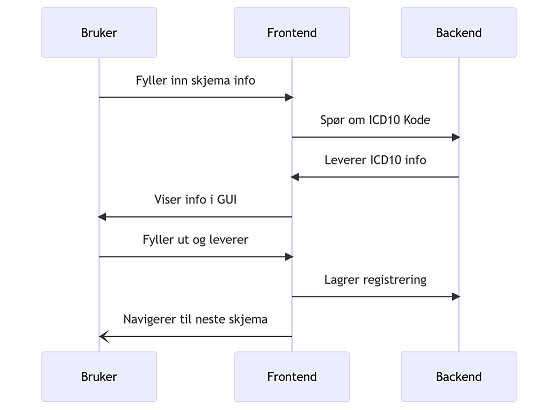
\includegraphics{images/sequence-diagram1.png}
\caption{Sequence diagram. Generert med mermaid.}
\label{fig:sequence-diagram}
\end{figure}

Utifra figuren kan vi se at hver gang et skjema som inneholder ICD10 koder eller andre eventuelle koder skal fylles ut vil prosessen stoppe tidlig og må ligge på vent til programvaren er oppdatert.

\subsection{Prosjektbeskrivelse og analyse}  

Utviklingen vil foregå i to ulike kode baser. Selve tjenesten som skal hente data fra eksterne kilder og i den eksisterende register koden der HTTP klient og midlertidig lagring av koder skal etableres.

\subsubsection*{Alexandria:} 
Applikasjonen vi skal utvikle har fått navnet Alexandria etter det store biblioteket i Alexandria i Egypt.

\subsubsection*{I eksisterende register kodebase:}

\begin{enumerate} 
    \item HTTP Klient som skal hente oppdaterte data fra Alexandria etter mottak om oppdaterte data 
    \item Storage service som lagrer og henter data fra in-memory database
    \item In-memory database
\end{enumerate}

\subsubsection*{Dataflyt i applikasjonen} 

%Figur - Dataflyt i applikasjonen
\begin{figure}[ht]
\centering
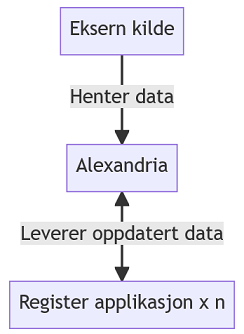
\includegraphics{images/dataflyt1.png}
\caption{Overordnet dataflyt i løsningen. Generert med mermaid.}
\label{fig:dataflyt1}
\end{figure}


\subsubsection*{Teknologier:}

Kvalitetsregister teamet bruker JVM teknologier for sin utvikling, da spesifikt Java og Kotlin, der hoved kode basen er en monolitt skrevet i Java som tar i bruk mange ulike teknologier. Ny kode skrives som regel i Kotlin. Tjenester som er ekstern til monolitten skrives i Kotlin. Med dette tatt i betraktning skal også denne tjenesten skrives i Kotlin. Alle nye tjenester kjører i kontainermiljø, der produksjonsmiljøet er driftet av Norsk Helse Nett (NHN).
Hele kvalitetsregisterplattformen til HN-IKT er i en migrering prosess der den skal over i Kubernetes. Det er derfor viktig at applikasjonen utvikles slik at den enkelt kan kjøre i et slik miljø.

\newpage
\subsubsection*{Hovedteknologier som skal brukes for tjenesten:}
\begin{itemize}
    \item Kotlin
    \item Ktor web server og http klient rammeverk
    \item R2DBC for databasetilgang
    \item Gradle som byggverktøy
    \item Docker og docker-compose for kontainer kjøremiljø og oppsett
    \item MySql database     
\end{itemize}

\subsection{Rammebetingelser}
 
Utvikling kan skje fra egen PC. Anbefalt å bruke IntelliJ IDEA for utvikling av Kotlin kode. Team for kvalitetsregister må gjøre tilgjengelig kildekode for utvikling av komponenter som er intern i register koden, eventuelt veilede i hvordan et eksternt lib kan opprettes slik det kan føyes inn i applikasjonen.